\subsection{\acl{pic}}\label{subsec:PIC}

\citet{PIC_2020} critize that dual branch, i.e. negative and positive sample sets, 
and epoch-based sampling strategies suffer from information leakage and 
the fact that individual instances are not visited frequently enough.
\ac{pic} is a one-branch method, i.e. only one random augmentation is applied to the input per iteration.
Moreover, \ac{pic} uses a sliding window based data scheduler 
as illustrated in \autoref{fig:pic_data_scheduler}
to ensure that the majority of instances are visited frequently.

\begin{figure}[!htb] % h = here, t = top, b = bottom, p = page of floats
    \centering
    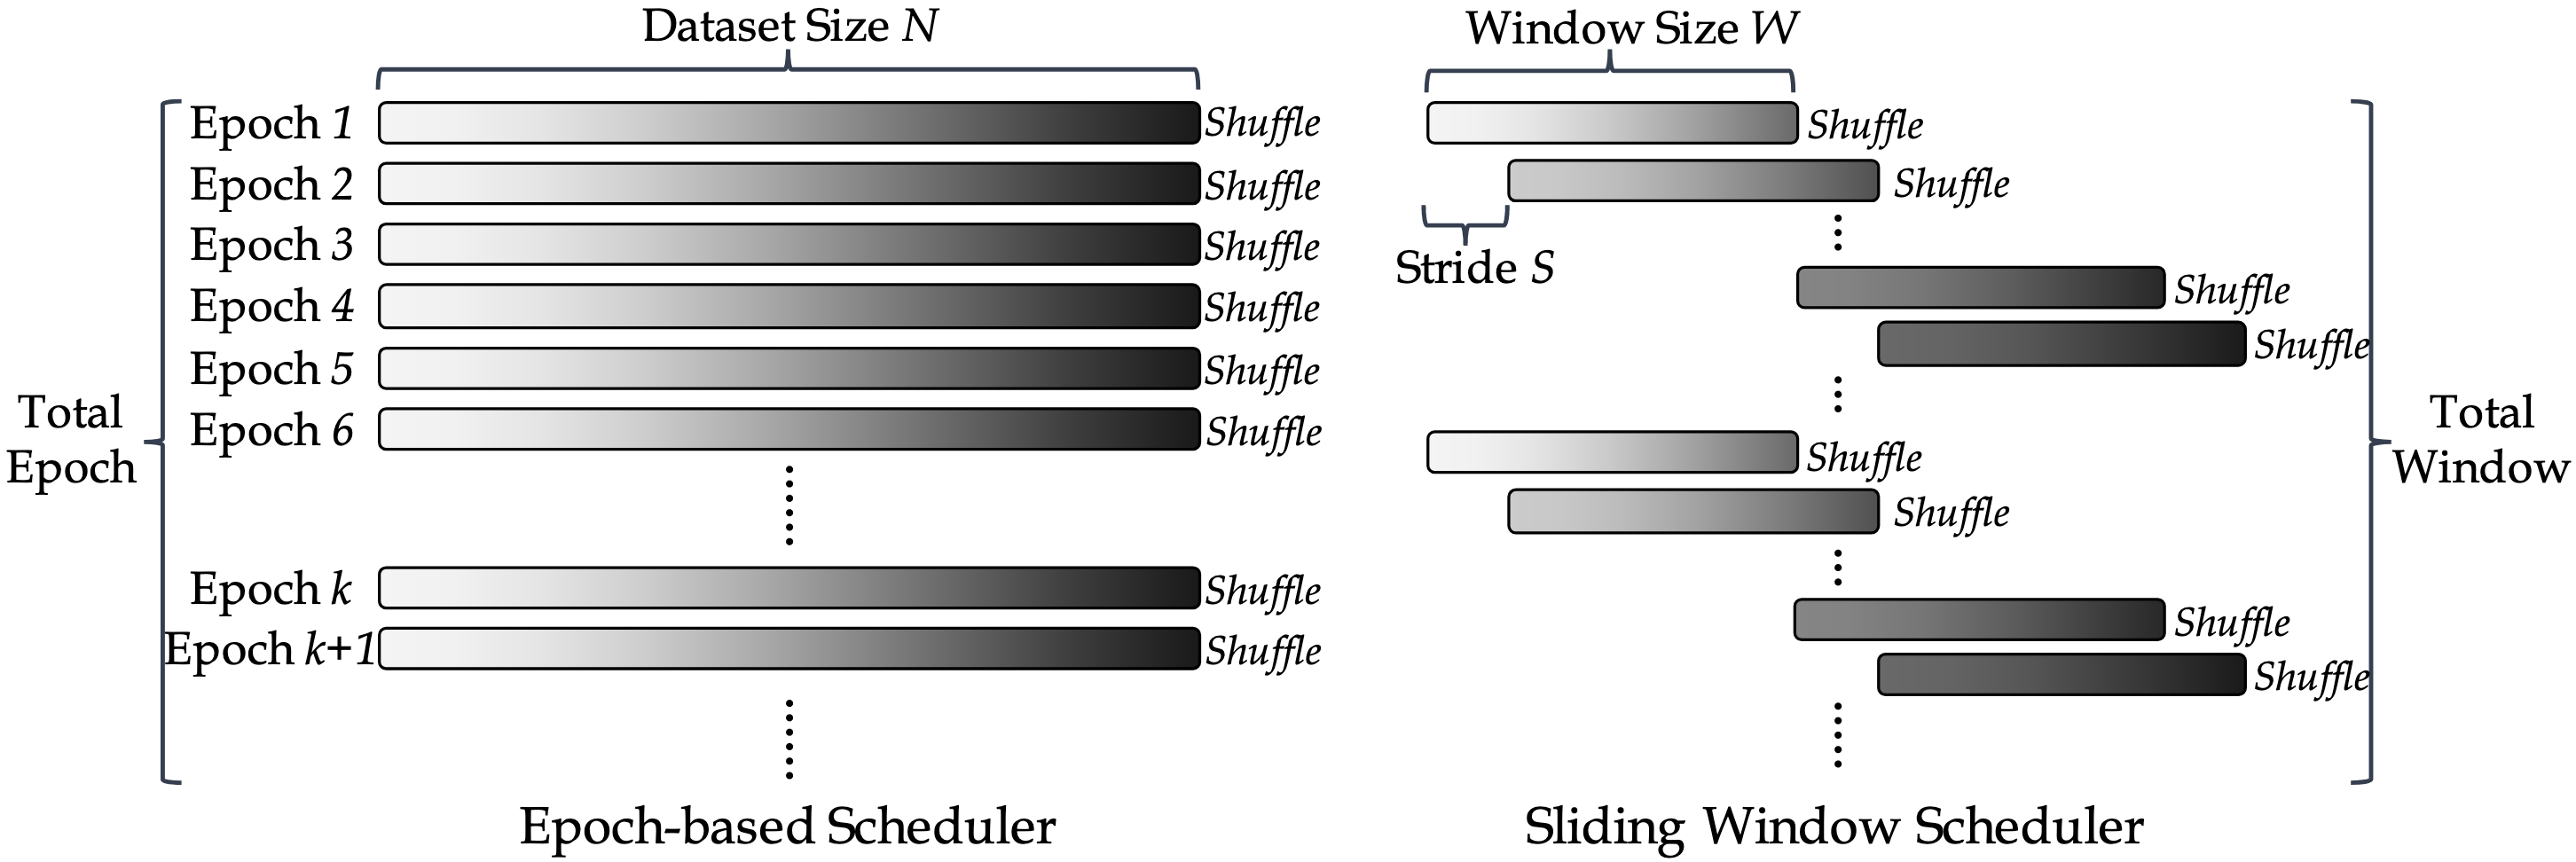
\includegraphics[width=300pt]{images/PIC_data_scheduler.png}
    \caption{Comparison of different data schedulers from \citet{PIC_2020}.
    While the epoch based version leads to long periods where instances are neglected in training,
    the sliding window approach ensures the majority of the instances are chosen more frequently.}
    \label{fig:pic_data_scheduler}
\end{figure}

% loss function
\citeauthor{PIC_2020} apply a cosine soft-max loss based on only the most recent $K$ instances 
to reduce computational costs.
